
\chapter{On Desacralization of Sanskrit}\label{chapter6}

\Authorline{Manogna Sastry and Megh Kalyanasundaram\footnote{pp xx-xx. In Kannan, K. S. (Ed.) (2019). \textit{Swadeshi Critique of Videshi Mīmāṁsā}. Chennai: Infinity Foundation India.}}

\begin{flushright}
\textit{\sf\em (manognashastry@gmail.com,}

\textit{\sf\em kalyanasundaram.megh@gmail.com)}
\end{flushright}


\section*{Abstract}

Among the primary themes Prof. Sheldon Pollock\index{Pollock, Sheldon} explores in his work, the relationship between culture and power in pre-modern India remains the linchpin of his arguments to build a case for many of his rather startling theories. Upon a closer examination of his thesis, one observes his proclivity to base ideas on a rather small subset of data, but build upon them sweeping generalisations that address the largest of questions. Thusly, Culture becomes equivalent to the set Language and to a narrower subset Literature – \textit{kāvya}\index{kavya@\textsl{kāvya}}. Similarly, even though he briefly mentions Power in context of \textit{rājya}\index{rajya@\textsl{rājya}} only once at the very beginning of his magnum opus \textit{The Language of Gods in the World of Men}, the former is not seen through the lens of traditional paradigms even once thereafter, but finds itself explored through anachronistic socio–political models of legitimation, socialisation and communication. His complete devaluation of the place and value of the \textit{pāramārthika}\index{paramarthika sat@\textsl{pāramārthika sat}}, his casual dismissal of the entire oral tradition that precedes written documentation, and hence, positioning \textit{kāvya} as something that was ‘invented’ at the beginning of C.E; his imperious assertion that ‘writing claims an authority oral cannot’ and its association with power while his seasonable use of linking the oral tradition of Vedic recital with oppression; his further dismissal of any metrical, thematic or lyrical creation that doesn’t fit his arbitrarily defined parameters for what constitutes \textit{kāvya}\index{kavya@\textsl{kāvya}}, all show a predisposition to select and fit time-honoured features of a native culture into his pre-defined models, of which the model of Desacralisation\index{desacralisation} of Sanskrit is one that the authors of this paper seek to explore.

\section{Introduction}

One of the great keys of the ancient Indian spiritual wisdom has been the recognition, understanding and development of a supremely profound relationship among the triptych – \textit{svarāj}\index{svarat@\textsl{svarāṭ}}, \textit{samrāj}\index{samrat@\textsl{samrāṭ}} and \textit{svadharma}\index{svadharma@\textsl{svadharma}}. To agnize the true nature of the Self, its sovereign power and truly master it – \textit{svarāj}; to discover and decipher the relationship between the Within and Without and hence mould and govern the world outside – \textit{samrāj}; and to do so, in harmony and concord with one’s own \textit{pneuma} and \textit{esse} – \textit{svadharma}, constitute the rungs of the triad, be it for an individual or for a collective. It is this \textit{svadharma} that lends the characteristic signature, especially to the collective soul and distinguishes it from other sets. One has seen this in what every culture has uniquely contributed to the progress of the human race. In the very choice and manner in which a culture frames its biggest questions and seeks to pursue them, one can see the distinctive traits of its peoples. If the ancient Graeco–Roman culture used the intellectual and mental planes as primary expressions of their marrow, India, in her odyssey, aspired not only for tellurian happiness of man but also sought the path to it through the loftiest and grandest of conceptions. The infinite world of the Spirit has been India’s domain to discover and manifest in forms that have been innumerably grand and precise and beautiful. As Sri Aurobindo\index{Sri Aurobindo} writes (Sri Aurobindo 1997:56),

\begin{myquote}
“India’s central conception is that of the Eternal, the Spirit here incased in matter, involved and immanent in it and evolving on the material plane by rebirth of the individual up the scale of being till in mental man it enters the world of ideas and realm of conscious morality, \textit{dharma}\index{dharma@\textsl{dharma}}. This achievement, this victory over unconscious matter develops its lines, enlarges its scope, elevates its levels until the increasing manifestation of the sattwic or spiritual portion of the vehicle of mind enables the individual mental being in man to identify himself with the pure spiritual consciousness beyond Mind. India’s social system is built upon this conception; her philosophy formulates it; her religion is an aspiration to the spiritual consciousness and its fruits; her art and literature have the same upward look; her whole dharma\index{dharma@\textsl{dharma}} or law of being is founded upon it.”
\end{myquote}

Any study of a culture needs to recognize the essential characteristics of its object of study, and it can be no different for studies about India. While canons and staggeringly huge volumes of works spanning the widest range of domains, including not only new creations but also penetrating and incisive analysis and commentaries — have been produced as a part of her oeuvre by her people, exchange and conflict with the Occident has seen, especially in the last millennium, interpretations and reviews that have often repeatedly painted radically different, and at times, inimical and hostile, pictures of India. In this time worn conflict, Europe, with its increasing turn towards and eventual consumption by materialism, has repeatedly cast its trademark lens to dissect and fractionate Indian tropes. The imperialistic hegemony it foisted across India and the rest of Asia typifies the pinnacles of its utilitarian and avaricious outlook. The peril this \textit{idée fixe} with materialism poses has taken new forms and shapes with the rise of capitalist America, which perpetuates the old order with new morphology.

Sheldon Pollock\index{Pollock, Sheldon} represents the best of this new affixation. In using models of power to analyse culture, Pollock does not venture too far away from his European predecessors, though his conclusions as seen in his work “Deep Orientalism\index{Orientalism}” and on the \textit{Rāmāyaṇa}\index{Ramayana@\textsl{Rāmāyaṇa}} are outright shocking and asinine. Through the theories he discards and templates he uses to construct the history – a new history – of Sanskrit, as well as his explicit motives that we will consider in this paper, Pollock clearly demonstrates his intent to see Asian phenomena explained in terms of parallels with European vernacularisation\index{vernacularisation} on the one hand and his construct of Cosmopolis – one clearly cannot escape the Greek/Latin significance of even this word – on the other, even though he professes to be the one who will give us a different theory of pre-modern India.

\newpage

If Pollock’s predecessors sought to Europeanise and thoroughly colonise the very character of India, Pollock himself seems determined to give us a version of our story that is cleansed of native, formative elements, separated as far away as possible from intuitive, instinctive features of our distinct culture and is replete with influences of the ‘good’ Outsider. One wonders if his learning of Sanskrit has no other purpose except to facilitate this irresponsible theorization.

The clash of ideas between the West and the East on what constitutes the sacred is a manifestation of the deeper lack of understanding between them about the fundamental difference that drives the very mind and soul of the two natures. There can be no doubt that some of the greatest achievements of the mind have emerged from Western thinking that has championed Intellect, Reason and Rationality – fine organs of the Mind. Western philosophies and her sciences, politics and economics are testament to this, while the models and categorization they employ bear this out repeatedly. For such a mind to recognize that a people seek to base their life on something that transcends its highest and most valuable force, requires a sincerity that is willing to set aside its passion and prejudice and approach that which is dissimilar to it. And, there have been several such sympathetic minds which have trod that path, be it Will Durant\index{Durant, Will} or Paul Brunton\index{Brunton, Paul}, or even Swami Vivekananda\index{Vivekananda, Swami} who powerfully carried the ideas of the East to the West. The eastern soul recognizes that the mind itself is an instrument of the Spirit. It champions man’s search for happiness beyond sensory and intellectual pleasures. It is this ethos that drives its external reflections as well, in her philosophies, religions, arts and sciences. This difference between the two approaches has at times led to enriching exchange of ideas and influences, just as there have been prolonged periods of clashes that have played out in arenas of the intellect and culture as well as that of the political and economic. What the West sees as sacred, what it considers corporeal and the separation between the two finds different base in the Indian thought process, where the \textit{pāramārthika}\index{paramarthika sat@\textsl{pāramārthika sat}}, \textit{vyāvahārika}\index{vyavaharika sat@\textsl{vyāvahārika sat}} and \textit{prātibhāsika} conceptions profoundly capture this distinction in a very MECE (mutually exclusive, collectively exhaustive) way, several millennia before McKinsey even coined the acronym.


\section{Desacralization\index{desacralisation} of Sanskrit}

In his 2006 book \textit{The Language of the Gods in the World of Men}, Pollock presents a picture of contrast between the use of Sanskrit in ancient India before and after the Common Era, separated by events purported to have occurred around the onset of the new millennium. His portrayal of ancient India is one that is boilerplate, charged with Brahmanical oppression and ritualization. He is determined in depicting Sanskrit as a language which had no worldly use apart from the sacerdotal, an especially absurd and unbelievable charge, considering the sheer range of work that exists in matters apart from sacred material from the period.

\begin{myquote}
“Sanskrit probably never functioned as an everyday medium of communication anywhere in the cosmopolis — not in South Asia itself, let alone Southeast Asia — nor was it ever used (except among the literati) as a bridge- or link- or trade language like other cosmopolitan codes such as Greek, Latin, Arabic, and Chinese. And aside from the inscriptions, which have larger purposes, there is little evidence that it was ever used as the language of practical rule; tasks such as chancery communication or revenue accounting seem to have been accomplished,” 

~\hfill (Pollock 2006:14).
\end{myquote}

Insisting that grammar was a tool of this hegemony, Pollock\index{Pollock, Sheldon} is very clear in establishing a temporal gulf between the use of Sanskrit for sacerdotal elements alone during BCE and for worldly affairs during the advent of the first millennium CE, even as he implicitly locates its origins outside India. The conception of a unity and ancient India’s philosophy, religion, arts and sciences and aspects of Life emerging from her chief pursuit of the Spirit is not even given a passing thought and thusly, Pollock creates a very bizarre picture of India’s past, where her chief pursuits for millennia seem to be exclusively limited to the religious and ritualistic. This intentional colouring with the sacred alone of India in BCE goes in tandem with Brahmanical oppression and excessive ritualization and its significance becomes apparent when Pollock uses this backdrop to focus on the non-sacred, liberating role of \textit{kāvya}\index{kavya@\textsl{kāvya}} during the CE. Thus, in Pollock’s work, it is never the co-existence of both, and percase sway of one over the other, but a clear absence of \textit{kāvya} in the earlier parts of BCE.

As one wonders how such a divide is possible in light of the composition of the epics and other luminous material including various \textit{śāstra}-s\index{sastra@\textsl{śāstra}} composed during the BCE period, Pollock renders a story where he considers the \textit{pāramārthika sat}\index{paramarthika sat@\textsl{pāramārthika sat}} and \textit{vyāvahārika sat}\index{vyavaharika sat@\textsl{vyāvahārika sat}}, chooses to focus – on the latter with a near complete disconnect between the two to the point of not admitting any influence of the former on the latter, while comparing them to Vico’s\index{Vico, Giambattista} concepts (Pollock\index{Pollock, Sheldon} 2006:2). With his interpretation that literature and non-literature were acutely separated from each other, Pollock mounts a case for treating literature and \textit{kāvya}\index{kavya@\textsl{kāvya}} as that which represented a clear break from the older order and heralded the beginning of the use of Sanskrit for worldly matters (Pollock 2006:5)

\begin{myquote}
“A sharp distinction between literature and non-literature was both discursively and practically constructed by those who made, heard, and read texts in premodern South Asia, and it is with that construction — out of a methodological commitment to \textit{vyāvahārika sat}\index{vyavaharika sat@\textsl{vyāvahārika sat}}, to taking seriously what they took seriously — that a history of their culture and power must begin.”
\end{myquote}

Not only is this idea manifestly ill-founded and wrong but, in Pollock’s work, sets the ball rolling for ascribing to \textit{kāvya}\index{kavya@\textsl{kāvya}} and \textit{praśasti}\index{prasasti@\textsl{praśasti}}, features that enabled to exaggeratedly desacralize\index{desacralisation} Sanskrit during the last centuries of BCE, and give him the platform to propound the Cosmopolis theory. His theorization is based on flimsy grounds as \textit{kāvya} is not as divorced from Veda\index{vedas@\textsl{Veda}-s} as Pollock would have one believe, though his peremptory tone is ever present (Pollock 2006:81)

\begin{myquote}
“Inscriptions, \textit{testimonia}, citations in literature, philology\index{Philology}, the history of literary theory—every piece of evidence hard and soft thus requires locating the origins of \textit{kāvya} in the very last centuries B.C.E., perhaps as much as a millennium after the Sanskrit language is believed to have first appeared in the subcontinent. Only an ideology of antiquity and the cultural distinction conferred by sheer age have induced scholars to move them back appreciably before this date—a move that requires conjecture every step of the way and the most fragile gossamer of relative dating.”
\end{myquote}

No doubt the themes and forms of \textit{kāvya} are \textit{laukika} too, but as seen from the traditionalist dating of the \textit{ādikāvya Rāmāyaṇa}\index{Ramayana@\textsl{Rāmāyaṇa}} itself, neither is it the invention of the new order in CE nor is it a tool of power in the manner of Pollock’s description.

The pattern of desacralisation\index{desacralisation} of Sanskrit in Pollock’s work thus begins with the clear demarcation between \textit{kāvya}\index{kavya@\textsl{kāvya}} and the sacred\index{vedas@\textsl{Veda-s}}, while characterizing the older Vedic order as oppressive and ritualistic; relying on oral transmission and grammar as agents of the exclusivity they sought to guard. With the advent of writing and \textit{kāvya}, the inventions of the new millennium in CE and the impetus provided by rulers who came from outside the Vedic order, Pollock believes Sanskrit was freed from the Vedic domination and could now be used by the common man. But what is more startling than these atypical hypotheses are the features Pollock\index{Pollock, Sheldon} attributes to the liberated, cosmopolitan Sanskrit – features of globalization\index{globalisation} – that enable him to make an open call for a secularized language that is cleansed of native, indigenous associations, and wearing only those intonations post colonialists such as Pollock see as convenient.

Desacralization of Sanskrit in \textit{The Language of the Gods in the World of Men} is problematic, right in the book’s Index. The detail for “\textit{desacralization of}\index{desacralisation}”, under the Index-item “\textit{Sanskrit language}” reads 62, 73-74, 74n70, 101, 170 (Pollock\index{Pollock, Sheldon} 2006:677). This is erroneous on two counts:
\begin{enumerate}[topsep=0pt]
\itemsep=0pt
\item “Desacralization” (or any of its forms) does not occur either on page 101 or in footnote 70 on page 74.

 \item “Desacralization” occurs in page 70, perhaps one of the more, if not the most important occurrences contextually, which is not indexed.

\end{enumerate}

These errors, which might be more typographical than intentional, of \textit{detailing that which does not exist} while \textit{missing that which exists}, is eerily symptomatic of Pollock’s scholarship about Sanskrit: detailing that which did not exist (or existed to an extent much lesser than what he would like one to believe) – the Political, while missing\textit{} or choosing to severely underplay that which exists – the Sacred.

The contexts of occurrences of “Desacralization” or any of its forms (Pollock 2006: 61-62, 69-70, 73-74, 170) are though, clear markers of Pollock’s theorization of the “Desacralization of Sanskrit language” and are strikingly relevant and revealing for this targeted \textit{pūrvapakṣa}\index{purvapaksa@\textsl{pūrvapakṣa}} effort. A thorough scrutiny of Pollock’s work — including identifying internal inconsistencies in his scholarship vis-à-vis his own positions, instantiating distortions through mistranslations or based on unsubstantiated claims, clear biases and dicey models — are aided by the findings in Malhotra (2006), with regard to desacralization, i.e. removal of the Sacred from Sanskrit. Rajiv Malhotra’s work (Malhotra\index{Malhotra, Rajiv} 2016: 126-127, 204-207) demystifies Pollock’s obfuscated writings, culminating in a neat tabulation ‘\textit{kāvya}\index{kavya@\textsl{kāvya}} theory milestone’ contrasting the ‘Tradition’s position’ with ‘Pollock’s position for the First Thirty Years’ and ‘Pollock’s\index{Pollock, Sheldon} Most Recent Position’ across epochs marked by the Veda-s\index{vedas@\textsl{Veda}-s}, \textit{Nāṭyaśāstra}\index{Natyasastra@\textsl{Nāṭyaśāstra}}, Abhinavagupta\index{Abhinavagupta} and Rupa Gosvāmin\index{Rupa Gosvami@Rūpa Gosvāmin} and outline the extent of ground already covered related to the study of the subject matter.

\section{Addendum: Further analysis of Desacralisation}

\subsection{Internal inconsistencies in data}

In the specific scope of Desacralization\index{desacralisation} of Sanskrit, two clear inconsistencies present themselves on close examination, their significance to his conclusions being almost self-evident.

\vspace{-.5cm}

\subsubsection{Restrictions – Yes or No?}

\vskip -5pt

Consider the very opening of Pollock’s Introduction to his book (Pollock 2006:1); in just the first three lines of the Introduction Pollock theorizes, or rather declares, in language quite emphatic and admitting to little doubt, that Sanskrit was definitely “restricted to religious practice” until it was “reinvented as a code for literary and political expression” during a specific “moment” — precisely, the beginning of the Common Era — and that the whole point of his book, rather his attempt, is to understand this “moment”, and another 72 pages follow with arduous topics and theorization – “\textit{Culture, Power (Pre)modernity}”, “\textit{The Cosmopolitan in Theory and Practice}”, “\textit{The Vernacular in Theory and Practice}”, “\textit{Theory, Metatheory, Practice, Metapractice}”, “\textit{Precosmopolitan Sanskrit: Monopolization and Ritualization}”, “\textit{From resistance to appropriation}”, “\textit{Expanding the Prestige Economy of Sanskrit}” – before inclusion of a statement about desacralization, that seems to clearly undermine Pollock’s own declaration in the first four lines of the Introduction:

\begin{myquote}
“It may ultimately be impossible to decide whether long-standing discursive restrictions rather than religious preferences explain the absence of Sanskrit from early Indian epigraphy, or whether recently arrived ruler lineages were the first to break with \textit{vaidika} convention and \textbf{desacralize} Sanskrit in the interests of a new cultural politics.” 

~\hfill (Pollock\index{Pollock, Sheldon} 2006:73)
\end{myquote}

\newpage

How exactly can one reconcile this belief with his earlier declaration that Sanskrit was long “\textbf{restricted} to \textbf{religious practice}”, which evidently becomes his basis and a prerequisite for that first ‘moment’ of transformation that he laboriously analyzes? Would Pollock hence at least concede that it may be proportionately “impossible to decide” whether his first “moment” of transformation really occurred the way he has proposed?

\vspace{-.4cm}

\subsubsection{Veda\index{vedas@\textsl{Veda}-s} and \textit{Kāvya}\index{kavya@\textsl{kāvya}} – Does Difference mean Discontinuity?}

After the above inconsistency, the chapters that immediately follow – “\textit{From Liturgy to Literature}” and “\textit{Literary Language as a Closed} Set” – is where Pollock locates bulk of his considerations specific to the “origin of” \textit{kāvya}, and in the process presents another clear inconsistency. Consider these two passages in adjacent pages:

\begin{myquote}
“To this degree, at least, it is correct to refer to \textit{kāvya} as the “direct descendant of the Vedic mantra\index{mantra@\textsl{mantra}}”…some commonalities with what preceded it must clearly be acknowledged” 

\vskip -5pt

~\hfill (Pollock\index{Pollock, Sheldon} 2006: 76)
\end{myquote}

\begin{myquote}
“Accordingly, if we are to grasp what premodern Indians understood by \textit{kāvya}—the \textit{vyāvahārika sat}\index{vyavaharika sat@\textsl{vyāvahārika sat}} of the term—and reconstruct its particular history, we must be careful to not make \textit{kāvya} a continuation of the Veda\index{vedas@\textsl{Veda-s}} by this worldly means and must avoid incautious generalization about its “Vedic effect”, to which much \textit{kāvya} anyway shows complete indifference.” 

\vskip -5pt

~\hfill (Pollock 2006: 77)
\end{myquote}

If a person endorses that \textit{kāvya} can, to some degree, be a direct descendant of Veda, with which it shares commonality, how can the same person suggest that one must be careful to not make \textit{kāvya} a continuation of Veda? A careful reading of the reasoning provided between the above two inconsistent positions, would show why it is less reasoning and more intellectual sleight:

\begin{myquote}
“In the Sanskrit critical tradition itself \textit{kāvya} came to be theorized as a species of discourse fundamentally different from the Veda, the consummate instance of this conceptualization being the account by the great synthesizer King Bhoja\index{Bhoja}, discussed below (section 3). Both theoretically and pragmatically the tradition drew a clear and untranscendable line dividing Veda from \textit{kāvya}, and in fact from every other kind of textuality. According to the influential tenets of Mīmāṃsā (the last centuries B.C.E.), the Veda was produced by no agent human or divine; as such, it cannot have any authorial intention (\textit{vivakṣā}\index{vivaksa@\textsl{vivakṣā}}, literally, desire to speak), which is a constitutive element of \textit{kāvya}. The same strong distinction between Veda\index{vedas@\textsl{Veda-s}} and \textit{kāvya}\index{kavya@\textsl{kāvya}} was made pragmatically, too. Before the modern era, the Veda was never read as \textit{kāvya}, never cited in anthologies, never adduced as exemplary in literary textbooks; in fact, the Veda was expressly denied to be \textit{kāvya}: “It is not the mere capacity for producing meaning as such that enables a text to be called \textit{kāvya}\index{kavya@\textsl{kāvya}},” argued the philosopher Abhinavagupta\index{Abhinavagupta} in the early eleventh century. “That is why we never apply the term to everyday discourse or the Veda.” This is so, as Sanskrit theory takes pains to point out, because \textbf{the rhetorical, discursive, aesthetic, and affective purposes of \textit{kāvya} are entirely different from those of the Veda.} Although Indian thinkers, like their Western counterparts, argued incessantly over how to frame an absolute and essential definition of this new and different kind of language usage—they were unsure whether this essence was to be located in figuration (\textit{alaṇkāra}\index{alankara@\textsl{alaṅkāra}}), style (\textit{rīti}\index{riti@\textsl{rīti}}), suggestion (\textit{dhvani}\index{dhvani@\textsl{dhvani}}), aestheticized emotion (\textit{rasa}\index{rasa@\textsl{rasa}}), propriety (\textit{aucitya}\index{aucitya@\textsl{aucitya}}), or something else altogether—they all agreed that it could be specified within a system of contrasts. It is something different from \textit{śāstra}\index{sastra@\textsl{śāstra}} (the discourse of systematic thought), from \textit{itihāsa} (accounts of the way things were), and from \textit{śruti}, the extant Vedic texts (those still available to be “heard”).” 

~\hfill (Pollock\index{Pollock, Sheldon} 2006:76) (\textit{emphasis ours})
\end{myquote}

\vskip 4pt

When carefully observed, one notices that the key conclusion from the above is the emphasized portion. Pollock’s sleight is in the fact that he uses the basis that proves ‘difference’, in order to propose and justify ‘discontinuity.’ A simple example should suffice to make the point: A daughter is certainly ‘different’ from her father; there certainly is a ‘clear and untranscendable line’ (of physicality, at the very least) between a daughter and father. Can the ‘difference’ however become proof to propose emphatically that the daughter is not a continuation of her father? Isn’t Pollock’s position, in addition to being inconsistent with another position of his own, also forced and unnatural?


\subsection{Instantiating Pollock’s Distortions}

Two instances of translation-related category-level distortions – distortions clearly visible when read vis-à-vis the account of unarguably one of the more credible (published) Insider voices of the twentieth century with regard to Sanskrit Literature, author of the seminal book \textit{History of Classical Sanskrit Literature viz.} M. Krishnamachariar\index{Krishnamachariar, M.} – are particularly striking and should be a clear indicator of Pollock’s motives. In addition to the two translation-related distortions, the distortions he induces about \textit{Writing, Orality} and \textit{Kavi}\index{kavi@\textsl{kavi}} are addressed.

\vspace{-.4cm}

\subsubsection{Translations of \textit{Śravya} and \textit{Dṛśya}}

Krishnamachariar’s\index{Krishnamachariar, M.} English translation of the terms \textit{Śravya} and \textit{Dṛśya}, in the context of one way of classifying \textit{kāvya}, is as follows: “\textit{Kāvya}\index{kavya@\textsl{kāvya}} is \textit{Śravya} or \textit{Dṛśya}, literally audible or visible” (Krishnamachariar 1937:79). For anyone from an Indian language speaking upbringing and with only an elementary Sanskrit knowledge, these translations – \textit{Śravya}\index{sravya@\textsl{śravya}}: Audible and \textit{Dṛśya}\index{drsya@\textsl{dṛśya}}: Visible – should be almost intuitive and hardly problematic. Note here that “Audible" and “Visible” are clearly mutually exclusive – they represent primarily, two distinct ways of perceiving, and reflect simply, nature as is visible to anyone willing to see it plainly.

Pollock’s English translations for these terms, and their context, make for interesting reading; for, it at once demonstrates not only a particular sleight in his method, ‘the \textit{Pūrvapakṣa}\index{purvapaksa@\textsl{pūrvapakṣa}} trap’ (to give his method a name), but also a clue of his underlying motive:

\begin{myquote}
“Consider first the old binary of Sanskrit literary theory — dating from the seventh century at the latest and never questioned in the tradition — that represents \textit{kāvya} as one of only two types, something seen (\textit{dṛśya}, i.e., drama) or something heard (\textit{śravya}, i.e., recitative);…” 

~\hfill (Pollock\index{Pollock, Sheldon} 2006: 84)
\end{myquote}

Before getting to the translation of \textit{Śravya} and \textit{Dṛśya} one finds in the quote above, the method he has employed here is quite remarkable. The whole quote, if one reads it carefully, is written in a form so that Pollock can claim that the quote is not his own s\textit{iddhānta}\index{siddhanta@\textsl{siddhānta}} but just his \textit{pūrvapakṣa}. In other words, Pollock gives the appearance that he is merely stating a fact from a tradition. While he does not make explicit his source, the greater sleight in his method is that as he builds the trap, by appearing to be simply quoting from a tradition, his own English translations of the categories are quietly sneaked in, in parenthesis. Given that Pollock does not make explicit in here his source, a common reader cannot actually check whether the translation is a motivated one or whether it is being faithful to the source from the tradition, the latter, a backdoor he appears to expertly build for himself even while the translations get an academic sanction. Yet, there are at least three hints to believe these translations might indeed be motivated or at least something he upholds, and not just a translation-consequence of a faithful \textit{pūrvapakṣa}\index{purvapaksa@\textsl{pūrvapakṣa}}: the translations also appear, outside the quote, in the Index; the phrase that completes the above quote – that “…there is no category for literature as something read.”; the actual translations of \textit{Śravya}: as “Recitative” and \textit{Dṛśya}: as “Drama”. Contrast Krishnamachariar’s intuitive translation for \textit{Śravya}\index{sravya@\textsl{śravya}} – Audible – with the translation Pollock has included – Recitative; while they may appear closely related when observed casually, they are actually markedly different. Including the distortion of \textit{Śravya} as Recitative (roughly, Oral) and \textit{Dṛśya}\index{drsya@\textsl{dṛśya}} as Drama allows Pollock to lend a certain impact to his \textit{Siddhānta}\index{siddhanta@\textsl{siddhānta}} – that “there is no category for literature as something read” – because \textit{Dṛśya}, having become ‘Drama’ instead of ‘Visible’, can effectively nullify any claim for tradition having factored in a category for ‘literature as something read’ (as ‘something read’ would certainly be encompassed in ‘Visible’); and \textit{Śravya}, having become ‘Recitative’ (i.e. roughly, Oral) provides the necessary contrasting context to something that is read. It is important to acknowledge here that translating \textit{Dṛśya} as Drama is not Pollock’s original handiwork. Yet, merely claiming innocence on that ground would hardly suffice, especially given Pollock is clearly aware of Krishnamachariar, whom he relegates, though, to a foot note.

\vspace{-.4cm}

\subsubsection{Translation of \textit{Mahākāvya}\index{mahakavya@mahākāvya}}

\textit{Mahākāvya} is translated as “Courtly epic” in Pollock(2006). The contexts of appearances of \textit{mahākāvya} in his book (Pollock\index{Pollock, Sheldon} 2006:70, 86, 98 - 99, 302-303) are quite revealing, such as in the case of translations of ‘\textit{Śravya}’ and ‘\textit{Dṛśya}’, where Pollock sneaked in, as demonstrated earlier, translations while appearing to be doing \textit{pūrvapakṣa}\index{purvapaksa@\textsl{pūrvapakṣa}} of a tradition, in the case of \textit{mahākāvya} too, he does something similar: again, without providing the specific source of what he has referred to as “credible tradition”, he sneaks in a translation of \textit{mahākāvya} – as “Courtly epics”. The extent of this distortion is easily grasped when the translation found in Pollock’s book is contrasted with the definition for \textit{mahākāvya} deduced in English, by an Insider such as Krishnamachariar\index{Krishnamachariar, M.}, from his translation of the characteristics of \textit{mahākāvya}, as specified by Daṇḍin\index{Dandin@Daṇḍin} in his \textit{Kāvyādarśa}\index{Kavyadarsa@\textsl{Kāvyādarśa}} and Viśvanātha\index{Visvanatha@Viśvanātha} in his \textit{Sāhityadarpaṇa}\index{Sahitya-darpana@\textsl{Sāhitya-darpaṇa}}. Krishnamachariar, in summarizing, writes:

\begin{myquote}
“Shortly stated, a \textit{mahākāvya} is a writing of considerable length, varying description and elaborate conclusion, embracing a narrative, theological or historical and is divided into Sargas or Cantos for convenience of narration. A poem that falls short of the several particulars that are required to make up a \textit{mahākāvya} is called \textit{laghukāvya}\index{laghukavya@\textsl{laghukāvya}} or a Minor Poem. Among these Minor Poems many are lyrical or didactic and these are treated in later chapter. In the following chapters, the history of poetry is traced by a chronological mention of writers of \textit{kāvya} and \textit{rūpaka.}\index{rupaka@\textsl{rūpaka}}” 

~\hfill (Krishnamachariar\index{Krishnamachariar, M.} 1937:81)
\end{myquote}

A direct association of \textit{mahākāvya}\index{kavya@\textsl{kāvya}} with “Court”, as found in Pollock’s scholarship, is conspicuously absent in an Insider’s translation from primary sources. The implication of characterizing \textit{mahākāvya} as\break “Courtly” seems to complement well, Pollock’s desacralization\index{desacralisation} agenda and not the least, his theorization about the so-called invention of \textit{kāvya}, but is clearly in variance with the characteristics of the \textit{mahā\-kāvya} as found in \textit{Kāvyādarśa}\index{Kavyadarsa@\textsl{Kāvyādarśa}} of Daṇḍin\index{Dandin@Daṇḍin}, who is acknowledged by Pollock\index{Pollock, Sheldon} himself, as being a key, influential part of Sanskrit \textit{kāvya} tradition. Sanctioning the translation of \textit{mahākāvya} as “Courtly epics” is distortive not only when compared to an Insider’s (Krishnamachariar) translation but also deviant from the translation of \textit{mahākāvya} as\break “poetry of the major form”, sanctioned by the author of “\textit{A History of Classical Poetry: Sanskrit—Pāli—Prākrit}”\textit{} (1984), Siegfried Lienhard\index{Lienhard, Siegfried}, to whom Pollock refers to, almost as an authority (at least whose history he deems as “standard narrative”), in fixing a date of a Sanskrit \textit{kāvya}, that date after which Pollock believes he can “say it unquestionably existed" (Pollock 2006:80). This deviation in translation from Lienhard is not an unimportant one because Pollock’s theorization of “a new secularization” (Pollock 2006:89) for \textit{kāvya} seems more like an extension of Lienhard’s characterization of the then prevalent atmosphere – “strong secular atmosphere” (Lienhard 1984:57)) – when ‘poetic activities’, according to Lienhard, shifted away from ‘Vedic poetry’, “a clear break in tradition between Vedic and classical poetry” (Lienhard 1984:57). Pollock’s extension, though, is typically Pollockian: that is extremist and being conclusive without conclusive evidence. The period of the so-called invention of \textit{kāvya}, which, for Pollock was conclusively a “cultural political transformation” (Pollock 2006:89), was for Lienhard, a period about which it was “scarcely possible to arrive at any definite conclusions" (Lienhard 1984:57).


\subsubsection{Writing in India before CE, Orality and the Sacred}

\vskip -3pt

Another example where Pollock is Pollockian, in the sense used above, is his conclusion about writing being imported into India in third century BCE (Pollock 2006:59,78,87). The importance and utter significance of this to Pollock’s theorization about the beginnings (according to him) of \textit{kāvya}\index{kavya@\textsl{kāvya}}, and to his history of Sanskrit itself, cannot be overstated. While he believes that writing in ancient India saw its beginnings during the times of the Mauryan chancery (Pollock 2006:81), Pollock states that the creation of \textit{kāvya} itself was possible because of the introduction of writing (Pollock 2006:83, 86). Pollock further historicizes kāvya and links with the “secularization” of Sanskrit language itself: 

\vskip 4pt

\begin{myquote}
“The point of historicizing the invention of \textit{kāvya}\index{kavya@\textsl{kāvya}} is not to gratuitously debunk claims to antiquity for Indian culture, as a certain old Orientalism\index{Orientalism} sought to do in a way that pained Indian intellectuals from an early date. It is to enable us to grasp the novelty of the cultural form, its place in the wider developments of culture and power in the Śaka- Kuṣāṇa era, and some of its meanings and effects, including a new secularization—not too strong a word, and no anachronism—of the gods’ language, a new medium, and a new cultural politics. The worldly transformation of Sanskrit made the language’s enormous expressive resources available for describing the world of human action; writing preserved its new products and made possible the dissemination of Sanskrit culture across vast reaches of Asia. The new order of culture and power, dimly visible in the fragmentary inscriptional record of the new dynasties of western and northern India, set the fashion for an unprecedented way of using Sanskrit for political and literary ends that would dominate in the centuries to follow. We need not go as far as Lévi and Sircar, though inscriptional evidence published since their day tends to confirm their arguments, and \textbf{not one new find has contradicted them.}” 

~\hfill (Pollock\index{Pollock, Sheldon} 2006:89) (\textit{emphasis ours})
\end{myquote}

\vskip 4pt

The last line of the last quote above is, again, quintessentially Pollockian. His claim, about inscriptional evidence post Lévi and Sircar, that ‘not one new find has contradicted them’ proves that either Pollock has not fully read Richard Salomon’s\index{Salomon, Richard} book of 1998 (from which Pollock quotes though) or he has wilfully chosen to not acknowledge/ignore findings (and theories thereof) – which Salomon has included – that might undermine his positions. In the chapter “\textit{The antiquity of writing in India of the historical period}” of his above mentioned book, Salomon, in writing about newly found evidence, writes:

\begin{myquote}
“However, a new body of material has recently come to light that seems to support the older theory that Brahmi\index{Brahmi@Brāhmī} existed before Mauryan times, that is, in the fourth century B.C. or possibly even earlier. This is a small group of potsherds bearing short inscriptions, evidently proper names, which were found in the course of excavations at Anuradhapura, Sri Lanka in strata which are said to be securely assigned by radiocarbon dating to the pre-Mauryan period. Various dates have been proposed for these graffiti, ranging from the sixth to the early fourth century B.C. The more recent publications on the subject have tended to favor the later date within this range, but in any case, these inscriptions still seem to show that Brahmi\index{Brahmi@Brāhmī} did indeed predate the Mauryan period.” 

~\hfill (Salomon 1998:12)
\end{myquote}

\begin{myquote}
“In conclusion, both the literary and the epigraphic evidence for the antiquity of historical writing in India are disappointingly inconclusive, since virtually all of the testimony is in one way or another vague or ambiguous. Probably the most cogent single piece of literary evidence for writing before the Mauryan period is Panini’s reference to script (lipi), although the uncertainties as to his date partially vitiate the value of this testimony….However, the recent discovery, mentioned above, of apparently pre-Mauryan graffiti in Sri Lanka has cast some doubt upon this point of view….Like other proponents of pre-Mauryan writing, Norman (279) attributes the absence of any surviving written records before the time of Asoka to the fact that early writing was primarily used for ephemeral documents. The practice of writing monumental inscriptions on stone was presumably an innovation of Asoka himself, possibly under the inspiration of the Achaemenian empire of neighboring Iran. Before Asoka, writing was probably used principally, if not exclusively, for economic and administrative, as opposed to literary and monumental, purposes; perishable materials such as palm leaves, tree bark, and (according to Nearchos) cloth, which have little chance of surviving the rigors of the Indian climate, were used. Thus, according to this view, we need not be surprised that no early specimens of Indian writing have survived, and their absence does not prove that they never existed.” 

\vskip -5pt

~\hfill (Salomon\index{Salomon, Richard} 1998:13)
\end{myquote}

\begin{myquote}
“In short, two schools of thought are dominant with regard to the problem of the antiquity of writing in historical India. One side sees no cogent archaeological or literary evidence for the existence of writing, and particularly of Brahmi script, before the Mauryan period. The other camp finds this hard to accept on pragmatic grounds, and moreover now sees archaeological evidence of pre-Mauryan Brahmi in the Anuradhapura graffiti, which are allegedly datable to the early fourth century B.C. at the latest. The issue remains unresolved, though it may be hoped that further discussions and examinations of the new evidence may ultimately lead to a consensus.” 

\vskip -5pt

~\hfill (Salomon 1998:14)
\end{myquote}

Even before Salomon’s 1998 book, Subhash Kak\index{Kak, Subhash}, in his 1994 paper makes some important observations about Brahmi\index{Brahmi@Brāhmī} script which Pollock\index{Pollock, Sheldon} surely would have found hard to reconcile with his narrative, if he had considered them:

\begin{myquote}
“The Brahmi\index{Brahmi@Brāhmī} script as seen in the earliest surviving records was systematic, reflecting the theories of Indian grammarians. Literary evidence as well as signs on early punch-marked coins suggests that writing in India during the second urbanization goes back much before the middle of the first millennium B.C. The punch-marked coins use a Harappan\index{Harappa} weight standard. The coins appear to have been originally issued as silver blanks by traders and their weights were checked by traders who put their own marks on the coins. By the sixth century B.C. the kings began putting their own issuing marks on the coins.” 

~\hfill (Kak\index{Kak, Subhash} 1994:2)
\end{myquote}

In a book published 21 years after his 1994 paper, Kak further obrserves:

\begin{myquote}
“According to B.B. Lal\index{Lal, B. B.}, some marks that are apparently in Brahmi on pottery in India go back to about 800 or 900 BC. The Indus script (also called Harappan or Sarasvati) was used widely during 2600-1900 BC. Its starting point has been traced back to 3300 BC and its use continued sporadically into the late centuries of the second millennium BC.” 

~\hfill (Kak 2015:82)
\end{myquote}

\begin{myquote}
“We know that writing was used in India prior to 500 BC. Written characters are mentioned in Chāndogya and Taittirīya Upanishad, and the Aitereya Āranyaka refers to the distinction between the various consonant classes. The voluminous Vedic texts also contain hints of writing in them. For example, Ṛgveda\index{Rg Veda@\textsl{Ṛg Veda}} 10.71.4 says…” 

~\hfill (Kak 2015:83) (\textit{diacritics as in the original})
\end{myquote}

Pollock’s heavy leaning on “scholarly consensus” (Pollock 2006:59) – which even the now-discredited Aryan Invasion Theory\index{Aryan Invasion Theory} had at one point of time – to support his chronological assumption regarding Brahmi syllabary, is symptomatic of one of his inherent biases, which he tries hard to mask, by claiming to be merely reading native sources — an effort which is, as is evident from the pattern of his scholarship, selective at best while being clearly insufficient and unscientific, given its heavy leanings on conjectural colonial chronology and its exclusion of results from truly modern fields such as 21st century archeology, DNA studies and computer-simulated literary astronomical evidence.

Asian countries have always valued orality as a powerful, faithful agent of not only knowledge dissemination but also a vehicle of cultural consciousness. The manner in which learning, from the oldest days of the Veda-s\index{vedas@\textsl{Veda}-s}, has been preserved, enriched and transmitted through oral forms is a singularly remarkable accomplishment, representing the Asiatic genius. While this mode of transference has been very coherently used across domains, including Vedic and \textit{śāstra}\index{sastra@\textsl{śāstra}} based creations, Pollock\index{Pollock, Sheldon} associates oral with the sole use for sacerdotal purposes alone and unconvincingly wields modern theories to project writing and introduction of the manuscript culture as the game changer that is simultaneous with the invention of \textit{kāvya}\index{kavya@\textsl{kāvya}}. By thus adding another feature to his clearly demarcated pattern – Vedic/Brahmanic/oral/oppression-ritualization/old order-in-BCE as that which marked the realm of sacred Sanskrit, Pollock\index{Pollock, Sheldon} holds writing as the liberating agent that helped bring Sanskrit to the realms of worldly use.

With \textit{kāvya} playing the role of introducing Sanskrit to usage in worldly domains, Pollock further narrows his already nominal and insufficient data and category set to a particular form of \textit{kāvya}\index{kavya@\textsl{kāvya}} viz. \textit{praśasti}\index{prasasti@\textsl{praśasti}}, the Indian panegyric. Crediting the introduction of the \textit{praśasti} to the influence of the Śaka-s\index{Sakas@Śaka-s}, the outsiders (who are the typical heroes in Pollock’s narrative), he begins the application of his trademark lens of power and its relation to culture to study the new role of Sanskrit in this non-sacerdotal world as well as its spread thus casting his seal on what constitutes a defining moment of change in the Indian history, when Sanskrit descended into the world of men from its sacred realms:

\begin{myquote}
“The history of the Sanskrit language and its social sphere has long been an object of interest to Sanskritists, for this is a curious history that holds considerable theoretical interest. The Sanskrit cosmopolis did not come into being simultaneously with the appearance of the Sanskrit language. Its development was slow and tentative, and for it to come about at all the very self-understanding of the nature and function of the “language of the gods,” as Sanskrit was known, had to be transformed. Chapter 1 delineates the circumscribed domain of usage and access that characterized the language from its earliest appearance in history to the moment when this field was dramatically expanded around the beginning of the Common Era. Ritualization (the restriction of Sanskrit to liturgical and related scholastic practices) and monopolization (the restriction of the language community, by and large, to the ritual\index{ritual} community) gave way to a new sociology and politicization of the language just around the time that western Asian and central Asian peoples were entering into the ambit of Sanskrit culture. Whether these newcomers, the Śakas\index{Sakas@Śaka-s} (Indo-Scythians) in particular, initiated these processes or simply reinforced those already under way cannot be determined from the available evidence. What is not in doubt is that it was then that a new era—a cosmopolitan era—began,” 

~\hfill (Pollock 2006:12)
\end{myquote}


\vspace{-.4cm}

\subsubsection{‘Nothing suggests’: How about the manuscripts, the destructions, the as yet unexcavated?}

“Nothing suggests” is a usage that punctuates some of Pollock’s\index{Pollock, Sheldon} key statements (Pollock 2006:79, 81, 86). While more than one thing and one person, at least those shown in 3.2.3 above, clearly suggest a date of Indic writing before 3rd century BCE, unless Pollock has read all manuscripts believed to be extant, “over thirty million” (Pollock 2006:558) of them, unless Pollock knows exactly all that has been destroyed in India, naturally or otherwise and unless Pollock knows all that is yet to be excavated, isn’t the usage ‘nothing suggests’ only too suggestive of Pollock’s “objectivity”?

\vspace{-.4cm}

\subsubsection{‘Kavi’:\index{kavi@\textsl{kavi}} Erased from the memory of Premodern South Asians}

In the beginning of the chapter where Pollock claims to chronicle the movement “from liturgy to literature”, Pollock makes these incredible declarations:

\begin{myquote}
“The beginnings of vernacular literatures are especially vexatious — in part because indigenist or nationalist thinking strives to find the deepest historical roots possible — and require separate theoretical discussion (chapter 8.1). But in the case of Sanskrit literature, too, most scholars resist acknowledging invention. Assuming the truth of the schoolmen’s tag \textit{ex nihilo nihil fit}, they have long sought to provide an infinitely receding history to Sanskrit \textit{kāvya}\index{kavya@\textsl{kāvya}}, or at least a very long genealogy leading back into the Vedic period. From one perspective — though it was one never adopted or even registered by people in premodern South Asia — Veda\index{vedas@\textsl{Veda}-s} and \textit{kāvya}\index{kavya@\textsl{kāvya}} do share certain traits. The ancient seers of the Veda are often referred to as \textit{kavi}\index{kavi@kavi}, the term later adopted for poet;” 

~\hfill (Pollock 2006:75)
\end{myquote}

Notwithstanding Pollock’s inconsistency in his position towards the “indigenist” – here a reason for vexation, whereas in ‘\textit{The idea of literature in Sanskrit thought}’ (Pollock 2003:41), a theoretical basis, a “turn” that “would seem to recommend itself easily” – Pollock declares that while “ancient seers of the Veda are often referred to as \textit{kavi}, this was hitherto not ‘adopted or even registered by people in premodern South Asia”. If this is not an incredible distortion – that people of premodern South Asians did not even register that ancient seers of the Veda were referred to as \textit{kavi} – what else is it? As counterintuitive this might seem to anyone familiar with \textit{Śrīmad Bhagavad Gītā}\index{Bhagavadgita@\textsl{Bhagavadgītā}}, and as ridiculous the need to disprove this with evidence might seem, here is one evidence: ‘\textit{kavi’}\index{kavi@\textsl{kavi}} is used to describe a Ṛgvedic\index{Rg Veda@\textsl{Ṛg Veda}} seer ‘Uśanas’\index{Usanas@Uśanas}, in the undoubtedly and incredibly popular South Asian, South East Asian, Indian text \textit{Śrīmad} \textit{Bhagavad Gītā}\index{Bhagavadgita@\textsl{Bhagavadgītā}} (10.37):

\begin{verse}
\textit{vṛṣṇīnāṁ vāsudevo’smi pāṇḍavānāṁ dhanañjayaḥ |}\\\textit{munīnām apy ahaṁ vyāsaḥ kavīnām uśanā kaviḥ ||}
\end{verse}

What is more, the word \textit{kavi} is translated as ‘poet’ in the translation of the same verse in book \textit{Bhishma} (Book 6, Volume 1) of Clay Sanskrit Library (CSL) (Cherniak\index{Cherniak, Alex} 2008), a library whose general editor is Sheldon Pollock\index{Pollock, Sheldon} himself, ironically. In the same CSL volume, the phrase “\textit{kaviṁ purāṇam}” (Cherniak 2008:231) is translated as “primordial poet” (Cherniak 2008:232). Now, unless one makes the laughable, certainly unsubstantiated, assumption that \textit{Śrīmad} \textit{Bhagavad Gītā} was not adopted or registered by Indian people in premodern South Asia, how can Pollock’s declaration – that those people did not adopt or register that ancient seers were referred to as \textit{kavi} - be considered tenable and not a distortion?


\subsection{\textit{Kāvya}\index{kavya@\textsl{kāvya}} in Veda\index{vedas@\textsl{Veda-s}} and \textit{Nāṭya\index{Natyasastra@\textsl{Nāṭyaśāstra}} Śāstra}: More evidence}

On the basis of the five points enumerated to expand on the topic \textit{Disconnecting Kāvyas from Vedas and Śāstras}, Malhotra concludes:

\begin{myquote}
 “Thus, Pollock tries to separate \textit{kāvya} from the Vedas. He says there is a ‘clear and untranscendable line dividing Veda from \textit{kāvya}’, and emphatically adds: ‘Before the modern era, the Veda was never read as \textit{kāvya}, never cited in anthologies, never adduced as exemplary in literary textbooks; in fact, the Veda was expressly denied to be \textit{kāvya}.’” 

~\hfill (Malhotra\index{Malhotra, Rajiv} 2016:130)
\end{myquote}

As a response to Pollock’s position, he then includes the following:

\begin{myquote}
“In response, K.S. Kannan\index{Kannan, K. S.} points out that the Atharva Veda makes a reference to \textit{kāvya} as something that never gets old, and never dies; the interpretations vary, some saying it is poetry, some saying it is the world that is metaphorically referred to. Kannan also points out that the Vedas have been designated as a \textit{kāvya} in some inscriptions. Lord Shiva is praised as the poet whose \textit{kāvya} is the triad of the Vedas, thereby implying that the three Vedas are Śiva’s \textit{kāvya}. Kannan has also compiled other extensive material to support this view. Also, traditional Hindu dancers performing Bharata Nāṭyam assert that their art is based on Bharata Muni’s \textit{Nāṭya Śāstra}\index{Natyasastra@\textsl{Nāṭyaśāstra}}, which in one of its first few verses (1.17) says it is based on Rig Veda\index{Rg Veda@\textsl{Ṛg Veda}}, Sāma Veda\index{Sama Veda@\textsl{Sāma Veda}}, Yajur Veda\index{Yajurveda@\textsl{Yajurveda}}, etc.” 

~\hfill (Malhotra\index{Malhotra, Rajiv} 2016:130)
\end{myquote}

To further expand the above corpus of evidence, and also in order to make available a ready reckoner for more detailed, actual textual analysis by traditionalists with expertise, 69 textual occurrences of the word \textit{kāvya}\index{kavya@\textsl{kāvya}} (and its forms) are compiled below, as found in Veda-s (\textit{Ṛg}\index{Rg Veda@\textsl{Ṛg Veda}}, \textit{Sāma}\index{Sama Veda@\textsl{Sāma Veda}}) and \textit{Nāṭya Śāstra}

\textbf{Eight occurrences in \textit{Ṛg Veda}:}

\textbf{1.83, 1.117, 1.121, 5.39, 8.8, 9.6, 9.97, 10.144}

Two occurences in \textit{Sāma Veda (Sāma Veda, Kauthuma Śākhā, 4th Prapāṭhaka, 1st Adhyāya):}

\vskip 4pt

\begin{verse}
\textit{vidhuṁ dadrāṇaṁ samane bahūnāṁ yuvānaṁ santaṁ palito jagāra} |\\\textit{devasya paśya kāvyaṁ mahitvādyā mamāra sa hyaḥ\break samāna} || \versenum{325}
\end{verse}

\vskip 4pt

\begin{verse}
\textit{pra kāvyam uśaneva bruvāṇo devo devānāṁ janimā vivakti} |\\\textit{mahivrataḥ śucibandhuḥ pāvakaḥ padā varāho abhyeti\break rebhan} || \versenum{524}
\end{verse}

\vskip 4pt

\newpage

\textbf{Fifty nine occurences in \textit{Nāṭya Śāstra:}\index{Natyasastra@\textsl{Nāṭyaśāstra}}}

\textbf{5.21, 5.108, 5.135, 7.7, 7.119, 7.125, 14.23, 15.227, 16.17, 16.42, 16.53, 16.88, 16.89, 16.92, 16.97, 16.116, 16.118, 16.119, 16.123, 16.128, 16.135, 16.172 17.41, 17.47, 17.57, 17.147, 18.5, 18.6, 18.9, 18.15, 18.23, 18.40, 18.42, 18.46, 18.50, 18.61, 18.96, 18.97. 19.32, 19.34, 19.53, 19.55, 19.66, 19.103, 19.105, 19.153, 20.22, 20.24, 20.29, 22.51, 25.88, 27.22, 27.26, 27.27, 27.33, 27.34,27.35, 36.35}

While 69 textual occurrences – 59 from \textit{Nāṭya Śāstra} and 10 from Vedas (\textit{Ṛg-}\index{Rg Veda@\textsl{Ṛg Veda}} and \textit{Sāman-}\index{Sama Veda@\textsl{Sāma Veda}}) – have been collated above to facilitate further analysis, already existing scholarship specific to poetry in Vedas, such as \textit{Atharvaved Ka Kāvya} and \textit{Sanskrit Kāvyaśāstra aur Kāvya Paramparā} by Radhavallabh Tripathi\index{Tripathi, Radhavallabh}, \textit{Devasya Kāvyam} by P.D. Mishra\index{Mishra, P. D.} could be relevant inclusions for further analysis.


\subsection{‘Category'cal omission: Upaveda\index{Upaveda}}

The category “Upavedas” is conspicuously absent, rather surprisingly, in Pollock’s\index{Pollock, Sheldon} work. The preeminent and globally renowned Insider to and practitioner of Sanatana Dharma\index{sanatanadharma@\textsl{sanātana-dharma}} tradition Pujyasri Chandrasekha\-rendra\index{Sarasvatī, Swami Chandrashekharendra} Saraswati Swami in his book \textit{Hindu Dharma}\index{dharma@\textsl{dharma}}, on the connection between Veda and Upavedas, wrote:

\begin{myquote}
“The Vedas\index{vedas@\textsl{Veda}-s} are of fundamental importance; the Angas and Upāngas derive their importance from them. Ayurveda\index{Ayurveda@Āyurveda}, Arthaśāstra\index{Arthasastra@\textsl{Arthaśāstra}}, Dhanurveda\index{Dhanurveda} and Gandharvaveda\index{Gandharvaveda@Gāndharvaveda} are called Upavedas\index{Upaveda}, subsidiary Vedas. The connection with the prime scriptures is thus obvious.” 

\vskip -5pt

~\hfill (Sarasvati\index{Sarasvati, Swami Chandrashekharendra@Sarasvatī, Swami Chandrashekharendra} 2008: 136)
\end{myquote}

The contents of Upavedas’ subcategory Gandharvaveda (in the chart titled “Caturdaśavidyāsthāna”, from his other book \textit{The Vedas}\index{vedas@\textsl{Veda-s}}) includes, among other key \textit{Kāvya}\index{kavya@\textsl{kāvya}} texts like \textit{Kāvyādarśa}\index{Kavyadarsa@\textsl{Kāvyādarśa}} of Daṇḍin\index{Dandin@Daṇḍin}, \textit{Kāvyālaṅkāra}\index{Kavyalankara@\textsl{Kāvyālaṅkāra}} of Bhāmaha\index{Bhamaha@Bhāmaha}, \textit{Kāvyamīmāṃsa}\index{Kavyamimamsa@\textsl{Kāvyamīmāṁsā}} of Rājaśekhara\index{Rajasekhara@\textsl{Rājaśekhara}}, also \textit{Śṛṅgāraprakāśa}\index{Srngara-prakasa@\textsl{Śṛṅgāra-prakāśa}} of Bhoja\index{Bhoja}, the one Pollock\index{Pollock, Sheldon} so extensively uses for his theorisation on \textit{kāvya}. Tradition’s view of the connection between \textit{kāvya} and Veda should be unambiguously clear.


\subsection{Pollock’s Use of Philology}

\vskip -5pt

Pollock’s writing is so well crafted, it leads one from sentences and thoughts that begin with ‘perhaps’, ‘maybe’ to those with disproportionately “definitive” conclusions, making even far-fetched and contrived notions mainstream. Charging a culture that has existed for several millennia with periods of exclusive, confining sacerdotal use of a language and then, a sudden liberating secularizing move, especially when there is voluminous material to show the absence of any such temporal schism, is truly remarkable for its sheer absurdity and vacuousness. There is no doubt that different forms have dominated different eras, with literature indeed being the prepotent form of a people’s expression of an age, and that is certainly justifiable and accountable, considering how the fundamental essence and ethos through all these expressive forms and manifestations remains unchanged. But then any analysis that refuses to consider the very basis and defining framework of the system under study but purports to answer huge questions deserves to be scrutinized for the purpose of such overcharging.

Pollock has always considered philology\index{Philology} an invaluable tool in studying the cultural and political conditions of the society, maintaining that critical philology can provide insights into creation of alternate models and theories, especially for pre-modern India, (Pollock 2006:36). Critical philology\index{Critical Philology} of his brand also sets the tone to enable him to read relationships between polity, kingship and \textit{praśasti}\index{prasasti@\textsl{praśasti}} (Pollock 2006:166) “No sooner had Sanskrit become the premier vehicle for the expression of royal will, displacing all other codes, than Sanskrit learning itself became an essential component of power. The figure of the learned king became quickly established, especially the king learned in Sanskrit philology\index{Philology} (and we may with justice speak of “philology” since “grammar” is often found to be used metonymically, standing for knowledge of lexicology, prosody, and the like, including literature). In fact, the topos of the educated king can be found in \textit{praśasti}\index{prasasti@\textsl{praśasti}} discourse across the cosmopolis.”

Placing the origins of philology in the Vedic world, Pollock\index{Pollock, Sheldon} believes all its features including metrics and language analysis heavily influenced Buddhist and Jain works whereas the flow of energies was never both ways. But the role played by philology assumes new heights in Pollock’s cosmopolitan order, as the former lays the basis for power, even as political power enabled the flourishing of philological traditions outside the realm of the sacerdotal and the liturgical. Citing classics such as the \textit{Rājataraṅgiṇī}\index{Raja-tarangini@\textsl{Rāja-taraṅgiṇī}} of Kalhaṇa\index{Kalhana@Kalhaṇa} and Kavibhoja’s\index{Bhoja} works, Pollock believes that philology with its tools of \textit{alaṅkāraśāstra}\index{Alankarasastra@Alaṅkāraśāstra} and \textit{praśasti} played a crucial role in furthering the political agency played by literary works. By the time this relationship weakened, Pollock believes the tradition of grammar assumed significance again, in the vernacular settings (Pollock 2006:368) “Given the powerful model of Sanskrit philology, with its full apparatus of grammars, dictionaries, treatises on the arts of literature (especially poetics and versification), and commentaries galore, a comparable set of instruments for disciplining and dignifying a language of Place was clearly essential if vernacularization was to be successful,” ensuring the connection between philology and the cosmopolitan order remains primary.


\subsection{The Nexus between \textit{Kāvya}\index{kavya@\textsl{kāvya}} and \textit{Rājya}\index{rajya@\textsl{rājya}}}

Remaining faithful to his own modus operandi of using small subsets to focus upon and extrapolating from them to making catholic statements about the whole domain, Pollock narrows down the relationship between \textit{kāvya} and \textit{rājya}, again a smaller subset of culture-power interaction, as his linchpin, “\textit{kāvya} and \textit{rājya} were mutually constitutive; every man who came to rule sought the distinction of self-presentation in Sanskrit literature, typically in the permanent public form of the \textit{praśasti”}\index{prasasti@\textsl{praśasti}} (Pollock 2006:18). This is fundamentally problematic as the idea of power, in spite of being a universal concept, finds different approaches across cultures. In India, the pursuit of the highest standards of living called for self–mastery as well as its external manifestation, in all domains including statecraft. The word power itself is a loose translation of \textit{śakti}, even though Pollock\index{Pollock, Sheldon} chooses to use the word \textit{rājya}\index{rajya@\textsl{rājya}}, which is a much narrower and specific subset. India has never been a country that has cast aside the role of power in the worldly affairs of man and has actively sought to give it a right and just structure by placing it in context of \textit{dharma}\index{dharma@\textsl{dharma}}, especially for men in positions of power, such as kings as seen in \textit{rāja-dharma}\index{raja-dharma@\textsl{rāja-dharma}}. What Pollock is interested though, is using his post-colonial lens of culture–power interaction, to analyse the relationship between \textit{kāvya}\index{kavya@\textsl{kāvya}} and \textit{rājya}. Having separated \textit{kāvya} from any connection to sacred elements and without studying \textit{rājya} in terms of native structures, Pollock wants to understand typical Western elements of “domination, exploitation, violence” that arise from power. 

Pollock believes that with the invention of \textit{kāvya}\index{kavya@\textsl{kāvya}}, and \textit{praśasti}\index{prasasti@\textsl{praśasti}}, ‘political orders’ defined in terms of their connection to produce literary texts underwent striking changes to reorient themselves and questions why the reordering entailed. Considering the politicization of culture, Pollock introduces (Pollock 2006:31) ‘two closely connected issues,’ concerning ‘the reproduction of power’ which he analyses through the lens of ‘legitimation of authority, ideology, hegemony, and like notions ‘ of Western social theories and ‘the constitution of power’. Setting up the Sanskrit Cosmopolitan order as the framework in which he would study the culture–power interaction, Pollock defines the order as being ‘territorially expansive,’ ‘politically universalistic,’ and ‘ethnically non-particularized,’ all notions that place Sanskrit on a global platform, even as he admits that territoriality and governance in the period remain indefinite concepts. Maintaining that the practice of political power was a practice in aesthetic form as well, Pollock believes (Pollock 2006:18) “that these aspirations were embedded in a set of cultural practices like \textit{kāvya} and \textit{praśasti}\index{prasasti@\textsl{praśasti}},” attributing to literature a specifically political role. Pollock himself remarks yet that defining a relationship between \textit{kāvya} and \textit{rājya} in the manner in which he has, presents ‘interpretative challenges’ and existing ideas from legitimation theories only represent,“The single available explanation of the social function of Sanskrit cosmopolitan culture is legitimation theory and its logic of instrumental reason: elites in command of new forms of social power are understood to have deployed the mystifying symbols and codes of Sanskrit to secure popular consent.”

Thus, in firstly defining a new relationship between two disparate entities and then trying to find explanatory models that would fit the relationship and in finding little of the same within existing theories, Pollock arrives at a point where he believes his cosmopolitan model is the most suitable template.


\section{Desacralisation\index{desacralisation} to Globalisation\index{globalisation} of Sanskrit}

Pollock’s\index{Pollock, Sheldon} tangled writing is rich in bold, sweeping generalisations with far reaching implications for several centuries of history, but what is more audacious is his confident assertions that he uses as starting points for his theories instead of established facts. There are lakhs of thousands of manuscripts, apart from the several thousand ones that were hauled away by the colonisers, that are yet to be collated and studied across the country to know more about the conditions in the past millennia, especially that of BCE. Any unbiased scholar would readily admit how one is short of material to make aberrant theorisations of the sort Pollock makes in considering the period of India over the last 2500 years. Pollock’s presumptuous statements include

\begin{myquote}
“The very act of permitting Sanskrit to speak openly in the everyday world was itself a decision (on the part of the Śakas among others) made against the backdrop of centuries of its public silence,” 

~\hfill (Pollock 2006:499)
\end{myquote}

\begin{myquote}
“Even as poets eventually decided to shatter this seclusion and produce expressive and other non-sacral texts in Sanskrit and, equally important, to commit them to writing, participants in many other areas of Sanskrit culture reasserted archaic practices of orality and exclusivity. It is especially when juxtaposed to such conceptions, moreover, that the first public inscription of political poetry in Sanskrit recovers the element of audacity, even scandalousness that made history. The cultural political act of the Śaka prince Rudradāman in the middle of the second century — which, if not actually inaugurating a new communications model, at the very least affirmed its acceptability and perceived efficacy in dramatic fashion — must accordingly be seen, like all the others, as a choice.” 

~\hfill (Pollock 2006:500)
\end{myquote}

It is incredible that the writer is so self-assured that he’s able to remark upon the Śaka-s'\index{Sakas@Śaka-s} “decision” of “permitting Sanskrit” to be spoken openly, against false claims of “centuries of its public silence,” and it becoming a representation of “the first public inscription of political poetry in Sanskrit recovers the element of audacity, even scandalousness, that made history,” all remarks that have such a strong tone to them, which is characteristically absent when Pollock adopts a language replete with “perhaps" and “maybe" and “suppose" while defining his data set. One can look hard in Pollock’s\index{Pollock, Sheldon} labyrinthine work trying to find solid, unassailable facts that can naturally lead one to his conclusions but come up with almost nothing.

Several Western Indologists have certainly held Sanskrit to be the chief vehicle for sacred purposes in the ancient past, but, there has been study of the use of the language for several \textit{vyāvahārika}\index{vyavaharika sat@\textsl{vyāvahārika sat}} disciplines as well, including the arts and sciences. But, none of this feature in Pollock’s scheme as non-sacral fields except the \textit{kāvya}\index{kavya@\textsl{kāvya}}, to which Pollock attributes the role of a great liberator. In trying to explain his dismissal of existing theories in favour of his incongruous models, Pollock casts aside ideas from modern social theories, legitimation and functionalism\index{functionalism}, all the while betraying his clear motive and intent to globalize\index{globalisation} Sanskrit.

In trying to justify his ictus on writing as characterizing the non-sacral nature of Sanskrit while he holds oral transmission as typical of the sacred old order, Pollock brings in the ideas of Niklas Luhmann\index{Luhmann, Niklas} to see how “cultural change and ideational change” is steered by technology, such as printing for instance. Pollock considers writing and the manuscript culture in context of ‘communication dissemination’ and sees it as propelling the spread of \textit{kāvya}, (Pollock 2006:498) “While admittedly remaining a cultural form that was fully realized only in public performance, \textit{kāvya} was created through the power of writing,” dismissing any connection between the oral tradition and \textit{kāvya}.

Such statements from Pollock, the Sanskritist, draw attention to the motives behind his wilful and explicit rejection of defining elements from the tradition while he tries to cover in ornate language and diffuse style of writing the absence of any substantial basis for his claims.

In considering ideas from modern social theory, Pollock traces the origins of linguism and the primeval role of language as “the core-factor in social–group identification” right upto the times of Dante\index{Dante}, Franz Rosenzweig\index{Rosenzweig, Franz}, Antonio Gramsci\index{Gramsci, Antonio} and Johann Herder\index{Herder, Johann} (Pollock 2006:505). Pollock then introduces Clifford Geertz’s\index{Geertz, Clifford} analysis of language being primordial to a culture in the sense of being a ‘first order “given” of social life’ and highlights his statements about India, as one where (Pollock 2006:506) “for some yet to be adequately explained reasons” the phenomenon was “particularly intense.” Pollock holds Geertz’ idea as an analytical concept that makes ‘social claims’ and not an ontological one, making a weak case comprising of a couple of lines that Geertz’s\index{Geertz, Clifford} category has sociological claim but not his conclusions, especially those that apply to linguism in India. Favouring Max Weber’s\index{Weber, Max} constructivist account over Geertz, including maintaining that it is the dominant position held among academics, Pollock presents the case that aids his narrative, (Pollock 2006:507) “primordial sentiment with respect to linguism (not his term, of course) is generated through the “cultural work” of elites, producing a “belief in the exclusiveness of [a] language community” that comes to seize the masses through the democratization of culture.” Using multilinguality and language plurality as evidence for the lack of a single ‘mother tongue’ for an individual in India, Pollock\index{Pollock, Sheldon} maintains that linguism was not native to pre-modern South Asia.

Even as one can give his theory credit to be able to hold some water in perhaps the second millennium of CE, one finds that it does not at all address the issues he speaks about in BCE as well as the first millennium of CE, a remarkably long period during which Sanskrit did function as the primary vehicle of thought and expression of an entire culture across a sub-continent. This methodology of Pollock, where he dismisses conflicting models even from European domains as those which are not native to Indian context and adeptly shifts the debate spatially and temporally to points of his own choosing in the grand narrative while seemingly trying to justify his positions is present across his work, making one wonder if it is wilful obfuscation.

In further considering theories from communication, socialization and legitimation, Pollock maintains,

\begin{myquote}
“Unwarranted generalizations based on European particulars pertain not only to the sociality of language but also to the place of culture as such in relation to power.” 

\vskip -5pt

~\hfill (Pollock 2006:511)
\end{myquote}

With no convincing explanation, Pollock dismisses with a casual mention the idea that Sanskrit could have been used for \textit{vyāvahārika}\index{vyavaharika sat@\textsl{vyāvahārika sat}} purposes and spread across the Indian sub-continent, calling the spread as a real ‘enigma’,

\begin{myquote}
“The weakest argument, and the most quickly dismissed, explains the role of Sanskrit across much of the cosmopolis but especially in Southeast Asia as driven by practical interregional communication needs. Unfortunately, there is no direct evidence that Sanskrit was ever used to fulfill these needs outside of certain scholastic and liturgical environments. There are undoubtedly some real enigmas here, such as Sanskrit’s massive invasion of the Javanese lexicon (upward of 40 percent, and penetrating to the most quotidian level), but these enigmas may be open to other kinds of solutions.” 

\vskip -5pt

~\hfill (Pollock 2006:512)
\end{myquote}

It is imperious of Pollock\index{Pollock, Sheldon} to not even consider the factual history of a country where for centuries it maintained trade and economic relations with several south Asian nations. Even an outsider such as Elphinstone has remarked upon the maritime trade of ancient India and the spread of Sanskrit culture across south Asia and dismissal of such genuine data will obviously lead to ‘enigmas.’ Such blatantly biased theorization, which would turn a blind eye to facts that paint a picture of a culture that embraced all aspects of life — sacral to non-sacral — so that one can create a temporal gulf between the two is what Pollock’s writing amounts to. And the resolution of these fantastic enigmas will surely emerge only through Pollock’s narrative.

The second functionalist argument that Pollock dismisses is the idea that Buddhists, Jains and outsiders turned to Sanskrit increasingly, after initially rejecting it, for its “technical precision.” Terming Sanskritisation\index{Sanskritization} as “a subset of social functionalism\index{functionalism},” Pollock spurns it as a theory that carries little merit,

\begin{myquote}
“Sanskritization is presented either as completely random or as a ceaseless process, without beginning or end, everywhere available to explain transculturation, as if Sanskrit culture were a higher form of life toward which lower forms inevitably aspire.” 

\vskip -5pt

~\hfill (Pollock 2006:514)
\end{myquote}

One wonders how a critic who goes by the label of a Sanskritist could express this veiled disdain for a culture that has been held as the touchstone for all of the Orient for millennia and a language that has been the torch bearer of its loftiest and most beautiful conceptions. Such criticism that passes in the name of academic analysis hardly justifies itself and can only inspire similar writing in defense. Pollock’s motive inspires a response Sri Aurobindo\index{Sri Aurobindo} rendered back in his own age (Sri Aurobindo 1997:316) –

\begin{myquote}
“The fit parallel to this motive and style of criticism would be if an Indian critic who had read European literature only in bad or ineffective Indian translations, were to pass it under a hostile and disparaging review, dismiss the \textit{Iliad}\index{Iliad@\textsl{Iliad}} as a crude and empty semi-savage and primitive epos, Dante’s\index{Dante} great work as the nightmare of a cruel and superstitious religious fantasy, Shakespeare\index{Shakespeare, William} as a drunken barbarian of considerable genius with an epileptic imagination, the whole drama of Greece and Spain and England as a mass of bad ethics and violent horrors, French poetry as a succession of bald or tawdry rhetorical exercises and French fiction as a tainted and immoral thing, a long sacrifice on the altar of the goddess Lubricity, admit here and there a minor merit, but make no attempt at all to understand the central spirit or aesthetic quality or principle of structure and conclude on the strength of his own absurd method that the ideals of both Pagan and Christian Europe were altogether false and bad and its imagination afflicted with a “habitual and ancestral” earthiness, morbidity, poverty and disorder. No criticism would be worth making on such a mass of absurdities, and in this equally ridiculous philippic only a stray observation or two less inconsequent and opaque than the others perhaps demands a passing notice. But although these futilities do not at all represent the genuine view of the general European mind on the subject of Indian poetry and literature, still one finds a frequent inability to appreciate the spirit or the form or the aesthetic value of Indian writing and especially its perfection and powers an expression of the cultural mind of the people.”
\end{myquote}

Harping back to his pet lens of power-culture relations, Pollock further charges,

\begin{myquote}
“The relations of culture and power so central to the choice to affiliate with the Sanskrit cosmopolitan order are entirely occluded; rarely is the general matter of cultural production even raised, let alone the specific question of what it meant to address a supralocal as opposed to a local audience in terms of either the sociality of the process or the aesthetics of the product. Emptied thus of both agency and the historical social worlds within which agency operated, the concept of Sanskritization\index{Sanskritization} ignores most of the critical aspects of the transculturation process; it has become a hindrance rather than a help to critical inquiry in the domain of literary-cultural change. Perhaps we should expect no more, however, for one can sift through the much deeper scholarship on Latinity (Romanization) and vernacularity and be equally disappointed.” 

~\hfill (Pollock\index{Pollock, Sheldon} 2006:514)
\end{myquote}

As highlighted earlier in context of his methodology, Pollock wonders why the kings of Khmer or people of Pagan wanted to adopt Sanskrit and having eschewed reasonable explanations, he bizarrely suggests the following,

\begin{myquote}
“Yet isn’t it possible that people conceive of political and moral needs in the first place through such visions as Brahmanism and Buddhism, that these are not instruments for filling needs but might in fact create them, and that their appearance in one place and not in another is a consequence of entirely contingent factors, such as the presence or absence of certain itinerant religious professionals?” 

~\hfill (Pollock 2016:515)
\end{myquote}

\newpage

Thus, Pollock finds theories that have been corroborated with facts over centuries unsuitable while peddling imaginative ideas such as these.

Considering ideas from legitimation theories, including those from Weber\index{Weber, Max}, Ricoeur, Guha and Giddens, Pollock states, (Pollock 2016:519) “It is patently false, for South Asia at least, that before the coming of colonial modernity there existed a single, unified, unblurred vision of either power or culture.” The concept of Dharma\index{dharma@\textsl{dharma}}, it must be said in reply, in all its forms and interpretations – Vedic, Buddhist, Purāṇic – as well as its manifestation seen across the \textit{śāstra-s}\index{sastra@\textsl{śāstra}} and canons including the \textit{arthaśāstra}\index{Arthasastra@\textsl{Arthaśāstra}} and \textit{rāja-dharma}\index{rajadharma@\textsl{rājadharma}}, has been uniquely Indian and pervasive in its spatial and temporal reach. Plurality in external forms of this core and defining essence of the Indian spirit has been an exemplary feature of the Indian culture. Dismissing the enormously congruent structures and templates that have existed not only to encompass but also master and subsume most aspects of the \textit{vyāvahārika sat}\index{vyavaharika sat@\textsl{vyāvahārika sat}} of the day, by stating that there is no common vision of a culture such as the Indian is outrageous and willful fabrication and misrepresentation.

Further maintaining that, (Pollock 2006:520) “ideology as we have always understood it—as a discourse that reproduces domination—is “simply irrelevant” for domination in agrarian societies,” when Pollock\index{Pollock, Sheldon} says, “Our concern throughout has been with \textit{vyāvahārika sat}, the subjective horizon of the actors involved,” it feels farcical because all he has done is disregard and overlook all relevant structures from within the tradition as well as historical evidence that undermine his theories while choosing to selectively retain elements from Western approaches. Repeating ad nauseum that \textit{kāvya}\index{kavya@\textsl{kāvya}} and writing were tools of desacralising\index{desacralisation} and unfettering Sanskrit from the domination of the Vedic oppression, Pollock sums up his case for rejecting prevailing Western models by declaring that models that present India primarily as a civilisation are hindrance to true analysis – while his own model that is entirely based on meagre data and inherent bias provides rare insight!

Pollock’s examination of the discourse on civilizationism is packed with arguments for rejecting any geographical claim over Sanskrit while he intends to see it globalized\index{globalisation}. Calling civilizationism ‘a conceptual and an analytical object,’ Pollock considers its interaction with nationalism, which is ‘a category of practice.’ Pollock characterises his approach as one which would (Pollock 2006:526) “isolate some key themes and tendencies and focus on some representative positions, concentrating on the evidence offered by literary culture.” However, instead of considering evidence from Indian tradition for instance, where the geographical beauty of the land has been beautifully captured in \textit{kāvya}\index{kavya@\textsl{kāvya}} to show that Sanskrit was not as rootless as he projects it to be or how the pluralism in India has been linked across time and age with the same essential ethos and belief systems, Pollock considers works of Herder, Fichte and the inapplicability of Heidegger’s\index{Heidegger, Martin} analysis to Sanskrit. Clearly detaching Sanskrit from any geographical bounds, Pollock states, (Pollock 2006:528) “Place was irrelevant in a cultural political formation that saw itself as existing everywhere in general and nowhere in particular.” Considering aspects of civilizationism, Pollock maintains that, (Pollock\index{Pollock, Sheldon} 2006:529) “To an outsider looking in at the field of Southeast Asian studies, the history of the civilization problem appears to fall into two major phases of conceptualization. The first is what we may think of as the colonial-European and Indian-chauvinist stage,” (notice the tone used, such as the word chauvinist, for the indigenous voice repeatedly in his work). Further, “On the European side, the Indianization\index{Indianization} of Asia was seen as an antecedent to its own contemporary imperial project; on the Indian side, it was taken as a consoling reminder of India’s own triumphant colonial past in the face of a humiliating colonized present,” (Pollock 2006:529).

Having maintained throughout the book that the spread of Sanskrit throughout Southeast Asia was never in material terms but through the agencies of the Brahmin priests who carried the language with its customs, Pollock now quotes French writers on India’s colonizing role in Southeast Asia, (Pollock 2006:529) “The French art historian Alfred Foucher\index{Foucher, Alfred} had argued in the 1930s that the Indianization of Southeast Asia was a matter not simply of influence but of “real colonization, in the full sense of the word.” French Orientalists evidently viewed what they interpreted as premodern colonization by Indians as a forerunner of their own well-known \textit{mission civilisatrice;} George Coedes\index{Coedes, George} actually spoke in terms of the “civilizing activity of India”,” while maintaining the following, (Pollock 2006:530) “The transculturation of Southeast Asia was the work of traders, adventurers, and itinerant religious entrepreneurs,” which in his own words, should indicate the presence of activities for which Sanskrit was used apart from the sacerdotal, for instance in trade. Clearly, Pollock wants to build a case for a purely sacerdotal tradition based period in the BCE and a sudden, desacralized\index{desacralisation}, globalized\index{globalisation} Sanskrit in the CE, even in the presence of evidence that would undermine his theory.

Further considering O. W. Walters\index{Walters, O. W.} work on Indianization\index{Indianization} in Southeast Asia, Pollock maintains that,

\begin{myquote}
“It is very hard, for the Sanskritist at least, to identify the slightest Cambodian inflection in the Sanskrit inscriptions Wolters analyzes beyond the occasional localism with respect to gender relations or sectarian practices (chapter 3.1). This is entirely expected, of course, since a principal function of the Sanskrit discourse was to efface local difference in favor of the transregional standard.” 

\vskip -5pt

~\hfill (Pollock 2006:513)
\end{myquote}

It is disconcerting indeed that the precision with which a language has been built is held with negative inflexion against it and instead, the language here is accused of ‘effacing’ regional standard, a charge which is baseless considering the sheer number and variety of vernaculars that existed along with Sanskrit in India itself. Having repeatedly ignored the fact that his theories are built on very little factual knowledge of pre-modern India, Pollock\index{Pollock, Sheldon} ironically remarks thus, (Pollock 2006: 531)“The assumption that a historical thought world can be separated from the historical language in which it is embodied.. is very hard to justify or even to comprehend. Like many other scholars, Wolters was inclined to take Indian literary allusions in inscriptions as mere veneer, decoration, and metaphorization,” (Pollock 2006:531), even as this statement becomes very true for his own work. Given the socio-political as well as the cultural conditions that existed in pre-modern India, as gleaned not just from the small data subset of \textit{praśasti}\index{prasasti@\textsl{praśasti}} but from several different sources across domains, Pollock’s models hold little water and his reading into the category of \textit{praśasti} and imputing it with extraordinary features of political power borders on the unbelievable.

Carrying forward his design for the case of a globalized\index{globalisation}, secularized Sanskrit, Pollock maintains that (Pollock 2006:532) “The foreign does not become such until civilizationalist thinking makes it so. Prior to that, the “foreign” is simply a cultural element circulating in the vast world, its origins undecidable and very likely irrelevant to the people who proceeded to make use of it,” sounding more like a line from a book that justifies intellectually imperialism and colonization. Further dismissing indigenism as a viable theory, Pollock remarks,

\begin{myquote}
“What the history of transculturation at work in the Sanskrit cosmopolis demonstrates every step of the way, however, is that all culture is really transculture. Indigenism is to the history of culture what creationism is to the history of the cosmos.” 

\vskip -5pt

~\hfill (Pollock 2006:533)
\end{myquote}

Even as Pollock presents a considerable body of work that has been undertaken in civilizational studies until current times, his own arguments for dismissing the theory, especially in the case of Oriental nations such as the Indian, replete with distinctive nature, are flimsy. His very questions, for instance, (Pollock 2006: 534) “What possible “conception of the world as a whole” could be said to characterize “Indian civilization,” which has witnessed struggles over conceptions of the world of the most incommensurable and irreconcilable sort for three millennia?” are incredulous, especially considering his caliber as a critic! Anybody with even a passable familiarity of Indic systems will recognize the uniqueness of its paradigms and templates with which it approaches matters, be it spiritual or worldly.

His declarations make more transparent his aims to globalize\index{globalisation} and secularise the language,

\begin{myquote}
“Indeed, a stable singularity called “Indian culture,” so often conjured up by Southeast Asian indigenists, never existed. What did exist was only a range of cultural and political codes and acts, many recently developed (Sanskrit \textit{kāvya}\index{kavya@\textsl{kāvya}}, public inscriptions, free-standing temple building, quasi-universalist political imagery, land-grants to Brahmanical communities, and so on) and undoubtedly generated out of various local practices,” 

\vskip -5pt

~\hfill (Pollock\index{Pollock, Sheldon} 2006:535)
\end{myquote}

\begin{myquote}
“Only gradually did all these practices coalesce into something like a cosmopolitan unity, one that was both “at home” and “abroad across this entire space. Not only is “Indianization”\index{Indianization} something of a empty signifier, since no unitary force ever existed to produce the process except in the trivial sense that the subcontinent provided one important source of new cultural flows to southern and eastern Asia; not only is it a crude sort of teleology, erroneously presupposing as cause what was only produced as effect; but equally remarkable, and almost always overlooked, is the fact that the Indianization of Southeast Asia was concurrent with, and no different from, the Indianization of India itself,” “From the processual perspective, “culture” or “civilization” (as in “Indian Civilization 101”) becomes nothing but an arbitrary moment illegitimately generalized, a freeze frame in a film taken for the whole story,” 

\vskip -5pt

~\hfill (Pollock 2006:539) 
\end{myquote}

As he dismisses any unifying thread that may have created the very existence of this range in the first place.

Considering that a critic of Pollock’s acclaim and scholarship makes these statements, one cannot but regard them not as objective scholarship, but an enormous philippic against India, replete with biased and motivated design.

Ironically, it is in Pollock’s summary dismissal of the applicability of Western theories to Indic studies that one finds the truest statements of the book, that deem apropos to his own work:

\begin{myquote}
“There is reason to doubt that culture is always and everywhere produced for the sheer legitimation of power, or for no social reason whatever but simply in the course of natural evolution,”

“Literature, the site where nations and regions and peoples insist on locating their real, continuous, primeval selves, may actually begin, and may do so by a process of continuous give and take from contiguous literatures. Present-day understandings of civilization may be based on indigenist conceptions that are unhistorical and reductive, while conceptions of the nation may be linked with views of culture in general that are anachronistic and simplistically functionalist. South Asian premodernity, and they in turn call that theory into question. If we are prepared to acknowledge the methodological fallacy of positing motives for action prior to determining those motives from the empirical materials, and if we can develop an openness to being surprised by the possible strangeness of the past, then we need to go back to the drawing board in trying to theorize the meanings of cosmopolitan and vernacular in South Asia before modernity.”

“It is instead a matter of resisting the prejudgments that such vocabularies entail, the categorizations that limit alternative possibilities, and the historical judgments based on accepting the terms of an argument that are inapplicable in the first place,” 

\vskip -5pt

~\hfill (Pollock\index{Pollock, Sheldon} 2006:564-565).
\end{myquote}


\section{Conclusion}

In continuing the tradition from his European predecessors of ignoring the viewpoints of the traditional scholar in framing models to study Indological elements, Pollock writes in \textit{What is South Asian Knowledge Good For}

\begin{myquote}
“Are there any decision makers, as they refer to themselves, at universities and foundations who would not agree that, in the cognitive sweepstakes of human history, Western knowledge has won and South Asian knowledge has lost? That the rest of the world is ineluctably becoming the West, not the South? That, accordingly, the South Asian knowledge South Asians themselves have produced can no longer be held to have any significant consequences for the future of the human species?” 

\vskip -5pt

~\hfill (Pollock 2014:4)
\end{myquote}

With such clear assertion of the victory of Western knowledge systems, one can only search in vain for a template that respects and actively considers the models and categorisations and studies from native, traditional systems, which, after all, constitute the very object under dissection.

A careful examination of Pollock’s oeuvre and especially the epilogue of \textit{The Language if the Gods in the World of Men} lays bare the man’s overtly political bias and intention to secularise and globalize\index{globalisation} Sanskrit — bringing under scrutiny his role of being the Sanskritist Outsider. Pollock wants to see Indian history cleansed of any overtly native connections with India’s past as he calls for a revised writing, with scholars such as himself deciding which elements are worthy of making it through their final cut. In trying to project a temporal gulf between what he portrays as a solely sacerdotal Sanskrit in the Vedic epoch to a purely desacralized\index{desacralisation} Sanskrit used in worldly domains, Pollock seeks to project newness in analysis which is factually hollow. For, the \textit{pāramārthika\index{paramarthika sat@\textsl{pāramārthika sat}} - vyāvaharika}\index{vyavaharika sat@\textsl{vyāvahārika sat}} categorization has always existed simultaneously from the ancient times, with copious works being produced in both realms; what Pollock achieves is the explicit highlighting of the former during one epoch and the latter during a later epoch, to suit his theorisations. Against the backdrop of his stated intentions, his dismissal of indigenism and civilizationism as valid, applicable theories assumes a more causal connection with his designs as against objective scholarly analysis. Consider his remarks,

\begin{myquote}
“Exhuming these anomalies as future potentialities, by decivilizing and denationalizing the Indian past where they were once lived realities, is something that might be achieved by a seriously historical account of Sanskrit in the world, one seeking not a return to roots but a “coming-to terms with our ‘routes,’” an unsentimental and nondefensive history, and one that is not merely, pointlessly erudite.” 

\vskip 3pt

~\hfill (Pollock\index{Pollock, Sheldon} 2006:580)
\end{myquote}

\vskip 4pt

Having begun the book with apparently modest aims of trying to understand a moment of rupture at the start of the CE, Pollock concludes by imperiously deciding that India indeed had a period where his Cosmopolitan model best captures the conditions of culture–power interactions, driven by literary inventions of the age such as \textit{kāvya}\index{kavya@\textsl{kāvya}} and \textit{praśasti}\index{prasasti@\textsl{praśasti}}, propelled by the bold impetus provided by the outsider kings. Have established his own imaginative vision of the past as the most authentic, felicitous, apposite and judicious model possible, Pollock openly laments the rise of forces in modern India that might not only challenge and debunk his claims but also revive Sanskrit studies in a manner that does not suit his project to declare Sanskrit a dead language that needs to be fossilized in a manner he sees fit.

\vskip 5pt

Pollock’s open hostility and detestation towards right wing political parties in India seems to hold more so for the modern Hindu who is unapologetically comfortable, if not proud, of his identity that is not shaped by the narratives of the colonizer or the oppressor, but seeks to revive his ancient spirit in a new light. His remarks,

\vskip 5pt

\begin{myquote}
“India, for its part, is hardly immune now to bad choices. The worst at present is the choice between a vernacularity mobilized along the most fragile fault lines of region, religion, and caste, and the grotesque mutation of the toxins of postcolonial \textit{ressentiment} and modernity known as Hindutva, or Hindu nationalism. The very names of the groups that make up the institutional complex of Hindutva—including the Bharatiya Janata Party (Indian People’s Party) and its ideological wing, the Vishwa Hindu Parishad (World Hindu Council)—bespeak what had never been spoken before, postulating in the one case a single Indian “peoplehood” \textit{( janata)}, in the other, Hinduism as an aggressive universalism. What is immediately clear from the history we have followed in the course of this book is that Hindutva is a perversion of India’s great cosmopolitan past, while the many new subnational movements (as in Assam and elsewhere) represent an entirely new, militant vernacularism, indeed, a kind of Heideggerization\index{Heidegger, Martin} of Indian life,” 

\vskip -5pt

~\hfill (Pollock 2006:575)
\end{myquote}

Crosses the lines of academic scholarship and objectivity and responses to his views too would have to be in a similar vein, even as one is surprised that such content is a part of academic discourse.

If Pollock\index{Pollock, Sheldon} is truly concerned about the interaction between local, cultural norms and global forces in modern times, and wishes to bring forth wisdom from the past, it would be a better project for him to study the horrendous impact of the excesses unleashed by West’s unbridled capitalism, instead of forcing unsubstantiated parallels with Europe, and tortuous and far-fetched theories on the role of \textit{kāvya}\index{kavya@\textsl{kāvya}} onto the historical narrative of the land. And Pollock’s distress at the rise of fundamentalist forces and need for secularist narrative as well would find a highly suitable subject in the repeated expressions of racist, xenophobic and sexist leanings in his own backyard of his country.

Indeed, it must be far easier to create and hand out these confounding conjectures to an unsuspecting people in the garb of academic writing than to watch with weariness the filling of the scale on the balance, even as one longs to cast aside all shackles of colonialism, in all its forms, and let the true voice of a people sing its own song.
\begin{myquote}
\textit{Afterwards came the night and a temporary end of all political initiative and creation. The lifeless attempt of the last generation to imitate and reproduce with a servile fidelity the ideals and forms of the West has been no true indication of the political mind and genius of the Indian people. But again amid all the mist of confusion there is still the possibility of a new twilight, not of an evening but a morning Yuga-sandhya. India of the ages is not dead nor has she spoken her last creative word; she lives and has still something to do for herself and the human peoples. And that which must seek now to awake is not an anglicised oriental people, docile pupil of the West and doomed to repeat the cycle of the Occident’s success and failure, but still the ancient immemorable Shakti recovering her deepest self, lifting her head higher towards the supreme source of light and strength and turning to discover the complete meaning and a vaster form of her Dharma\index{dharma@\textsl{dharma}}.} 

\vskip -5pt

~\hfill (Sri Aurobindo\index{Sri Aurobindo} 1997:444)
\end{myquote}

\section*{Appendix A}

\textbf{2. Categories that belong to the province of \textit{Kāvya}\index{kavya@\textsl{kāvya}} proper, as found in Lienhard’s\index{Lienhard, Siegfried} 1984 book}
\begin{figure}[H]
\centering
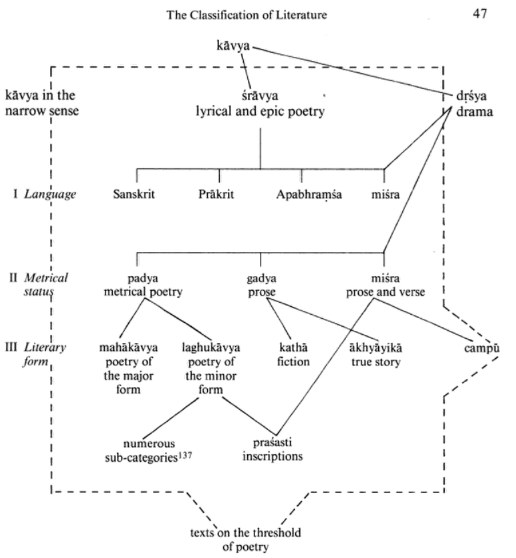
\includegraphics[scale=.52]{images/chapter8/image1.png}
\end{figure}

\section*{Bibliography}

\begin{thebibliography}{99}
\bibitem{chap8-key01} Cherniak, Alex. (2008). \textit{Mahabharata Book 6 Bhishma Vol 1.} Edited by Isabelle Onians, General editor: Sheldon Pollock. New York University Press and the JJC Foundation.

 \bibitem{chap8-key02} Elphinstone, Mountstuart. (1841). \textit{History of India. Vol. 1.} Second Edition. London: John Murray.

 \bibitem{chap8-key03} Griffith, Ralph T.H. (1896). \textit{Rig Veda.} \url{www.sacred-texts.com/hin/rigveda}. Accessed on Nov 12, 2016.

 \bibitem{chap8-key04} Kak, Subhash. (1994). “The Evolution of Early Writing in India”. \textit{Indian Journal of History of Science.} Vol. 29(3). pp 375--388.

 \bibitem{chap8-key05} —. (2015), \textit{The Wishing Tree – Presence, and Promise of India.} New Delhi: Aditya Prakashan.

 \bibitem{chap8-key06} Krishnamachariar, M. (1937). \textit{History of Classical Sanskrit Literature.} Madras: Tirumalai-Tirupati Devasthanams Press.

 \bibitem{chap8-key07} Lienhard, Siegfried. (1984). \textit{A History of Classical Poetry: Sanskrit—Pali—Prakrit Vol. III} Fasc. 1. Wiesbaden: Otto Harrassowitz.

 \bibitem{chap8-key08} Malhotra, Rajiv. (2016). \textit{The Battle for Sanskrit.} New Delhi: HarperCollins Publishers.

 \bibitem{chap8-key09} Naik, Ashay. (2016). “The Peculiarity of the Pollock Challenge”. \textit{Swarajya Mag}. \url{www.swarajyamag.com/culture/the-peculiarity-of-the-pollock-challenge}. Accessed on Nov 12, 2016.

 \bibitem{chap8-key10} Pollock, Sheldon. (2001). “Death of Sanskrit”. Comparative Studies in Society and History. Volume 43, Issue 2 April 2001. pp. 392--426. 

 \bibitem{chap8-key11} —. (Ed.) (2003). \textit{Literary Cultures in History}. Berkeley: University of California Press.

 \bibitem{chap8-key12} —. (2006). \textit{The Language of Gods in the World of Men}. Berkeley: University of California Press.

 \bibitem{chap8-key13} —. (2014). “What is South Asian Knowledge Good For?”. \textit{South Asia Institute Papers} ISSUE 01 2014 4. 4. 2014. pp 01--22.

 \bibitem{chap8-key14} Salomon, Richard. (1998). \textit{Indian Epigraphy}. Delhi: Munshiram Manoharlal.

 \bibitem{chap8-key15} \textit{Sāma Veda Saṁhitā Kauthuma Śākhā}. \url{https://www.sanskritdocuments.org/doc_veda/sv- kauthuma.html?lang=sa}.

 \bibitem{chap8-key16} \textit{Nāṭya Śāstra}. \url{https://www.sanskritdocuments.org/sanskrit/by-category/natyashastra.php}. Accessed on Nov 12, 2016.

 \bibitem{chap8-key17} Sarasvati, Chandasekharendra. (2008). \textit{Hindu Dharma – The Universal Way of Life.} Mumbai: Bharatiya Vidya Bhavan Bhavan‘s Book University.

 \bibitem{chap8-key18} Sri Aurobindo. (1997). “The Renaissance in India and Other Essays on Indian Culture”. \textit{The Complete Works of Sri Aurobindo – Volume 20.} Pondicherry: Sri Aurobindo Ashram Publications Department.

 \end{thebibliography}

